% !TeX spellcheck = en_US
\documentclass[./main.tex]{subfiles}
\begin{document}
\subsection{Web Architecture}
\subsubsection{Reason on implementing a Web Client}
As the application has its target user in the 
administrative world, it was decided that 
a web will be created alongside the mobile application that will
make the usage of our services easier to our customers
in administrative environments. It has been decided that the 
mobile app can be really useful for doing little 
tramits, for chatting with some customers, for 
quick searches of products/services and enterprises...\\
But it has been felt that in order to make it more usable and
accessible for administrative porposes a web client
should also be created.
\\\\
Furthermore, the implementation of the web client 
shined some light on how to communicate with the backend
and has lead us to iterate a little bit on the API endpoints
that were implemented on the last sprint. This is nice because now
on the third sprint the integration of the mobile app with the 
backend will be a lot more straightforward.
\subsubsection{React}
For implementing this Web Client React has been used, which is a 
library built in javascript for creating User Interfaces. 
To be more precise React was used because it gives the opportunity
of working with Hooks. Hooks are functions that comprehend inside them inmutable
components with independent states, wich makes the code a lot more
clean and structured and simplifies the amount of chaos that has
to be dealt with usually when it's programmed with vanilla javascript.
\\\\
Also React has a huge community, and it has a lot of libraries that
have been key for making a lot more easier the programming task.
Some examples can be:
\begin{itemize}
	\item react-router-doom
	\item react-modal
	\item redux-react-session
	\item react-bootstrap
	\item ...
\end{itemize}
\subsubsection{Redux}
In this part of the project, redux has also been used. In fact a react library
called redux-react-session that builds a store to maintain the state of our session is being used.
Also it creates the correspondig Session Cookie to maintain the value of the authorization token
provided by our backend. This way, every time a request that needs authorization has to be made,
it will be possible to pass the value of the token stored in the browser cookie within the request .
\subsubsection{Web Client Architecture}
By the moment the Web Client is still in a development phase, so for 
now the default testing server that React provides to us is being used.
Although, a nginx+docker is expected to be used when deploying our application
to a production enviroment.
\\\\
Right now the application is able to fully connect with the backend,
beeing able to Register, SignUp and interacting with all the different 
features that our application provides.
\\\\
Also, the chat has been implemented using websockets. For doing so, we used a React library called 
react-use-websocket that has been used as a wrapper of the complexity of connecting with the client websocket to the server.
\subsubsection{Web Client Project structure}
\begin{figure}[H]
	\centering
	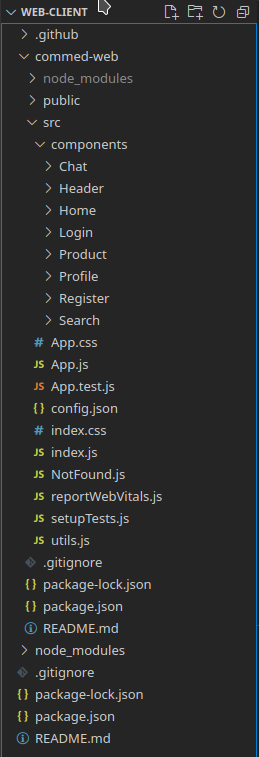
\includegraphics{img/web-client-project.png}
	\caption{Project Structure}
	\label{fig:redux}
\end{figure}
The project has been divided in different folders and components based on the different features that the application have. Each component will have its own independent js and css file. The application has been designed following a hierarchical model for the different components that can be seen in the next diagram:
\begin{figure}[H]
	\centering
	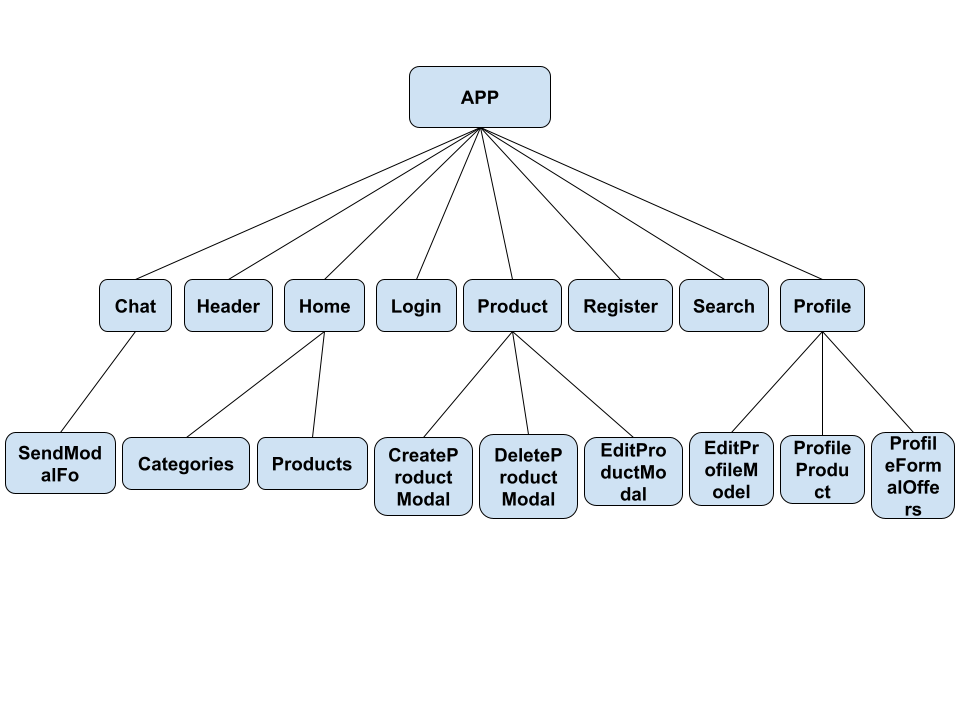
\includegraphics[width=0.8\textwidth]{img/React-tree.png}
	\caption{Project Structure}
	\label{fig:redux}
\end{figure}
Each one of the components will maintain his own state. This will make the thins a lot more tidy and in order. Also, some child components inherit some of the state of their parents. This is because a change done in a child component maybe have to be reflectet on the parent component. 
\subsubsection{Challenges}
The management of files and images in the front and in the communicatios with the backed has 
been a really challenging topic. For doing this, different approaches had been tryed and finally
we decided to pass the images encoded in base64 with in the json request.\\
The first aproach that was tryed was using the form-data Content-Type. We didn't succeed on parsing in the backed the 
information that was beeing send using this protocol so we decided to switch. 
After some more attempts and a lots of ours of search for solutions. We found that a possibility was sending
the images in b64 and then decode those images and parse them into Django FormFields.
\\\\
Another Challenging topic has been the chat. As we have different kinds of messages, wee had to agree
in a protocol with the backend for retrieving the informations of the messages. Also, the implementation
of the comunication through the web socket was not trivial, keeping the chats updated at real time with 
all the events that happen.
\\\\
Finally, one of the biggest challenges has been making the web usable. This includes making the web responsibe,
with all the components that had been developed separetly nicely connected. As we said in our idea presentation,
we want to build a really confortable expirience to the user, showing there that our application
really makes it's live easyer. Eventhough we put a lot on effort on this, a lot of work is still remaining in this
part. 
\end{document}